\documentclass{article}
\usepackage[T1]{fontenc}
\usepackage{hyperref}
\usepackage{amsmath}
\usepackage[utf8]{inputenc}
\usepackage[polish]{babel}
\usepackage{graphicx}
\usepackage{amsfonts}
\usepackage{placeins}


\setlength{\textheight}{21cm}

\title{{\bf Zadanie nr 4 - Przekształcenie Fouriera, Walsha-Hadamarda,
kosinusowe i falkowe, szybkie algorytmy}\linebreak
Cyfrowe Przetwarzanie Sygnałów}
\author{Dominik Gałkowski, 247659 \and Jan Śladowski, 247806}
\date{10.06.2025}

\begin{document}
\clearpage\maketitle
\thispagestyle{empty}
\newpage
\setcounter{page}{1}
\section{Cel zadania}
    Celem zadania jest zapoznanie się z operacjami transformacji sygnałów dyskretnych
    przy użyciu wybranych metod oraz zaimplementowanie ww. operacji transformacji
    w programie z zadania trzeciego.
\section{Wstęp teoretyczny}

Na podstawie instrukcji do zadania 4,
        do programu z zadania trzeciego zostały dodane funkcjonalności
        możliwości rysowania wykresów sygnałów dyskretnych o
        wartościach zespolonych w postaci dwóch wykresów o wspólnej
        dziedzinie. Wykresy są umieszczone jeden nad drugim oraz
        zostało przyjęte założenie, że sygnały zespolone będą tylko
        wynikiem transformacji Fouriera, więc będą prezentować funkcje
        w dziedzinie częstotliwości.
        Zostały zapewnione dwa tryby wyświeltania wykresu:
        \begin{itemize}
            \item (W1) – górny wykres prezentuje część rzeczywistą
                amplitudy w funkcji częstotliwości, a wykres dolny
                część urojoną
            \item (W2) – górny wykres prezentuje moduł liczby
                zespolonej, a dolny argument liczby w funkcji
                częstotliwości
        \end{itemize}
        Ponadto zostały zaimplementowane transformacje przedstawione
        poniżej: 
        \begin{itemize}
            \item dyskretna transformacja Fouriera - algorytm z
                definicji o złożoności O($N^2$), gdzie wyliczenie
                każdej próbki wyniku wymaga wymnożenia i zsumowania
                wszystkich próbek sygnału wejściowego przez
                odpowiednie, wyliczane na bieżąco wsþółczynniki
            \item dyskretna transformacja Fouriera - algorytm szybki w
                miejscu (\emph{in situ}) z decymacją w dziedzinie
                czasu (DIT FFT) o złożoności O(Nlog(N)), nie wymaga
                alokacji dodatkowej pamięci na bufor próbek podczas
                obliczeń, ponadto wszystkie współczynniki są wyliczone
                przed obliczeniami w tablicy o długości równej połowy
                długości bufora próbek
            \item dyskretna transformacja kosinusowa typu drugiego -
                algorytm z definicji
            \item dyskretna transformacja Walsha-Hadamarda - algorytm z
                definicji
            \item dyskretna szybka transformacja Walsha-Hadamarda -
                algorytm szybki
        \end{itemize}

\section{Materiały i metody} 
    Pierwszym krokiem w czasie dokonywania eksperymentów było wygenerowanie trzech sygnałów
        sinusoidalnych. Ich równania zostały przedstawione poniżej:
        \begin{figure}[h!]
            \centering
            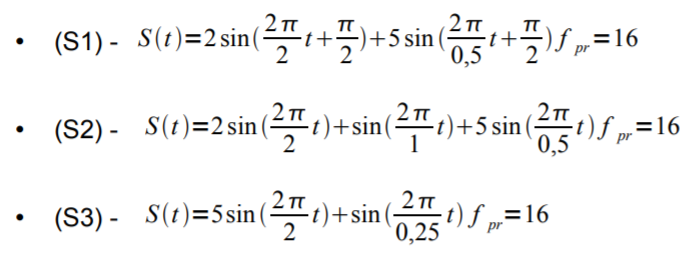
\includegraphics[width=0.7\textwidth]{img/equations.png}
        \end{figure}
        Następnie zostały przeprowadzone dla każdego z nich transformaty przedstawione poniżej:
        \begin{enumerate}
            \item Dyskretna tranformacja Fouriera z definicji
            \item Dyskretna tranformacja Fouriera wariant szybki
            \item Transformacja kosinusowa z definicji
            \item Transformacja Walsha-Hadamarda z definicji
            \item Transformacja Walsha-Hadamarda wariant szybki
        \end{enumerate}

        Wyniki transformat zostały przedstawione poniżej łącznie z wykresami sygnałów oznaczonych
        symbolami S1, S2, S3. 

\section{Eksperymenty i wyniki} {
    \subsection{Sygnał S1} 

        \begin{table}[h!]
            \centering
            \begin{tabular}{|l|l|l|}
                \hline
                Czas początkowy & \shortstack{Czas trwania \\ sygnału} & \shortstack{Częstotliwość\\ próbkowania}   \\ \hline
                0 & 16s & 16Hz         \\ \hline
            \end{tabular}
            \caption{Parametry wejściowe dla sygnału S1}
        \end{table}

        \begin{figure}[h!]
            \centering
            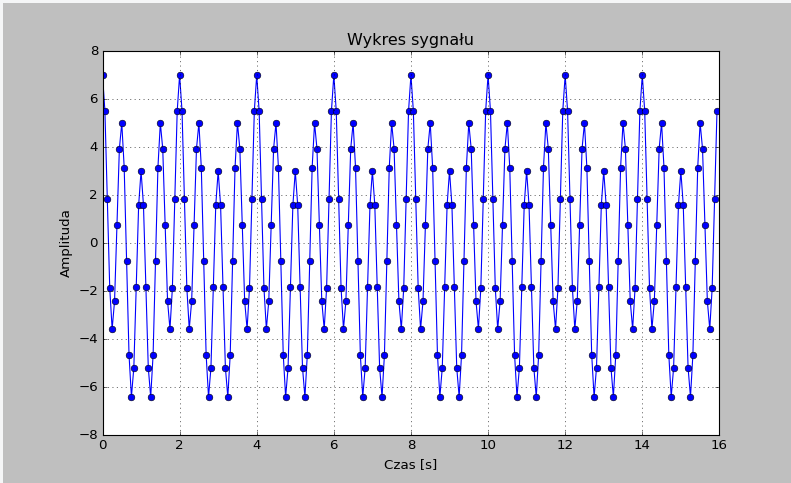
\includegraphics[width=\textwidth]{img/S1.png}
            \caption{Wykres sygnału S1}
        \end{figure}
        \FloatBarrier

        \subsubsection{Dyskretna tranformacja Fouriera z definicji}

                \FloatBarrier
                \begin{figure}[h!]
                    \centering
                    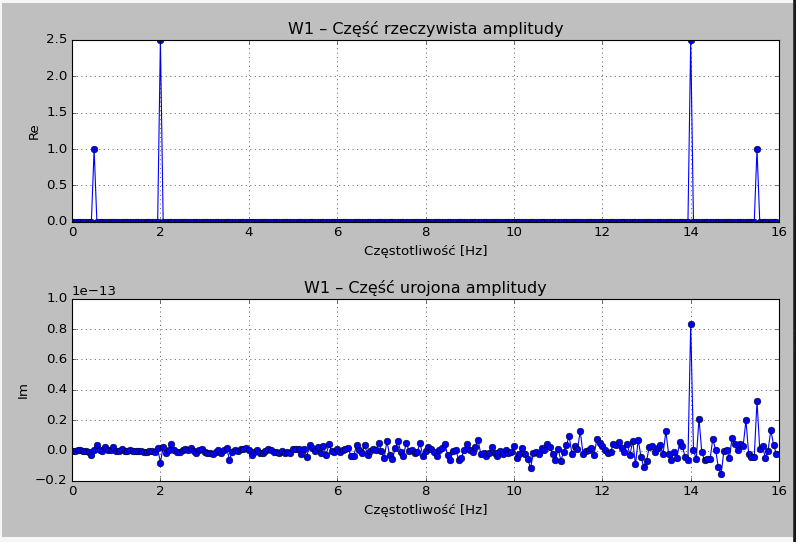
\includegraphics[width=1\textwidth]{img/w1s1.png}
                    \caption{Wykresy W1 dla sygnału S1}
                \end{figure}

                \begin{figure}[h!]
                    \centering
                    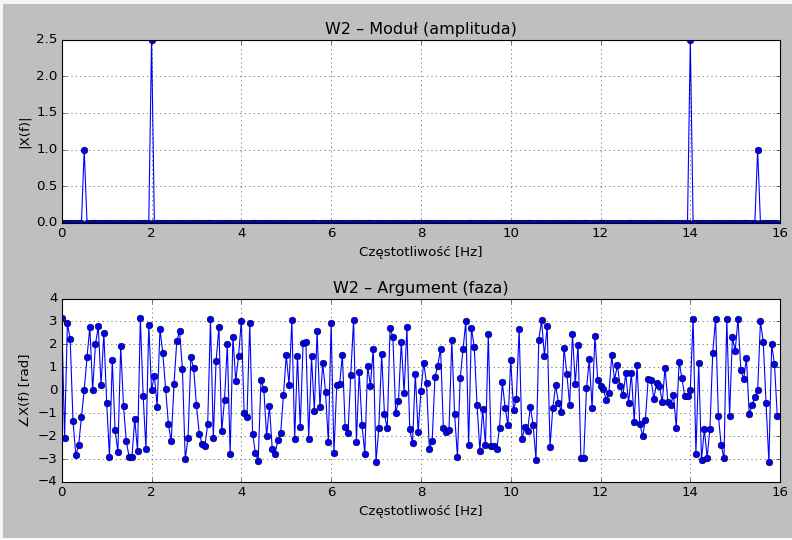
\includegraphics[width=1\textwidth]{img/w2s1.png}
                    \caption{Wykresy W2 dla sygnału S1}
                \end{figure}
                \FloatBarrier

                Czas wykonania obliczeń (s): 0.020

        \subsubsection{Szybka tranformacja Fouriera}

                \FloatBarrier
                \begin{figure}[h!]
                    \centering
                    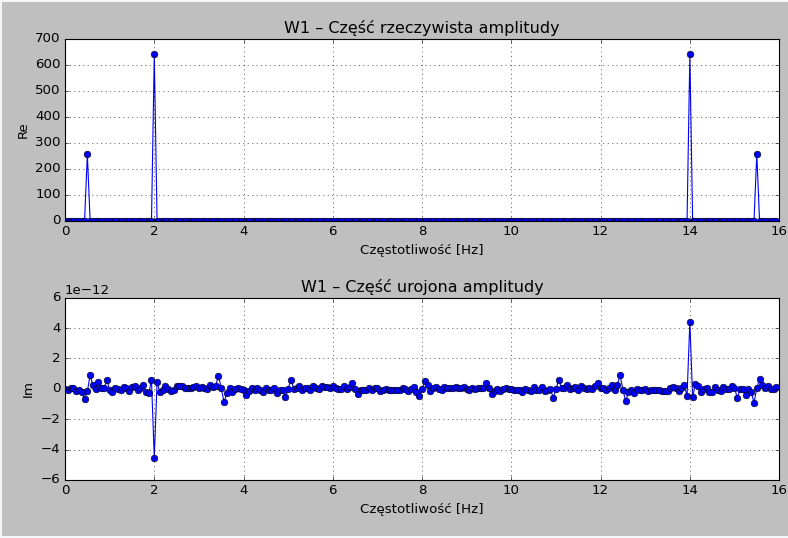
\includegraphics[width=1\textwidth]{img/w1s1_2.png}
                    \caption{Wykresy W1 dla sygnału S1}
                \end{figure}

                \begin{figure}[h!]
                    \centering
                    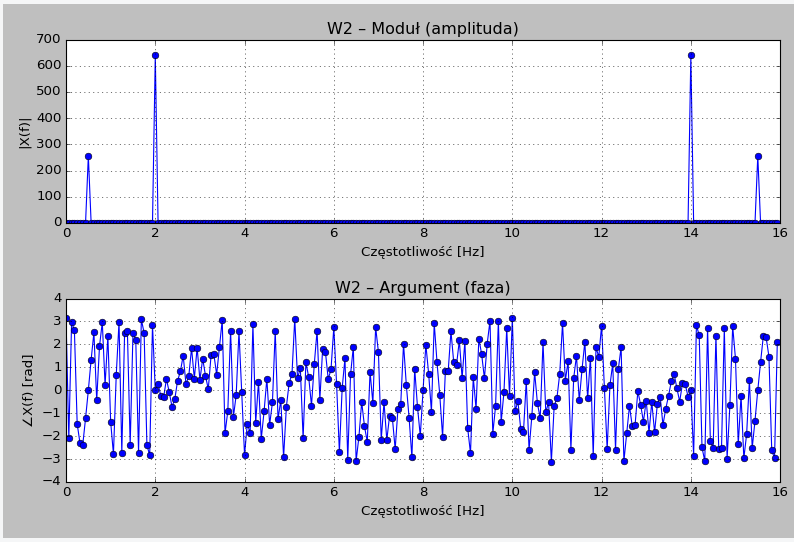
\includegraphics[width=1\textwidth]{img/w2s1_2.png}
                    \caption{Wykresy W2 dla sygnału S1}
                \end{figure}
                \FloatBarrier

                Czas wykonania obliczeń (s): 0.002

            \subsubsection{Transformacja kosinusowa z definicji}

            
                \begin{figure}[h!]
                    \centering
                    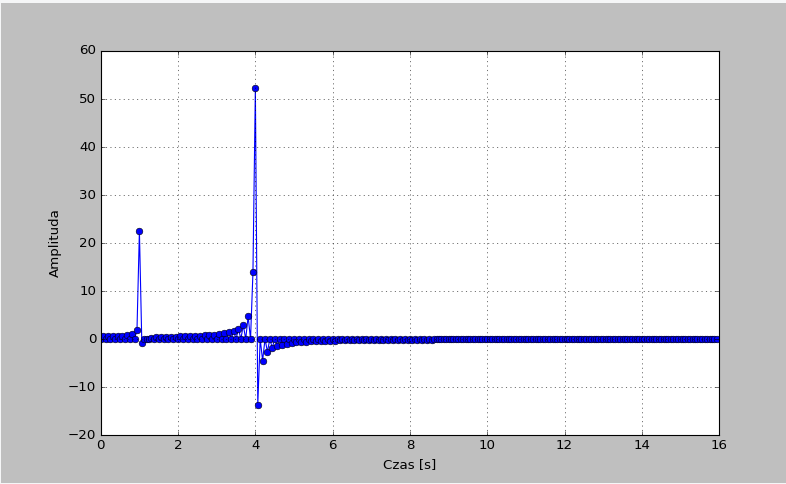
\includegraphics[width=1\textwidth]{img/dcts1.png}
                    \caption{Wykresy dla sygnału S1}
                \end{figure}
                \FloatBarrier

                Czas wykonania obliczeń (s): 0.045
            
            \subsubsection{Transformacja Walsha-Hadamarda z definicji}

            
                \begin{figure}[h!]
                    \centering
                    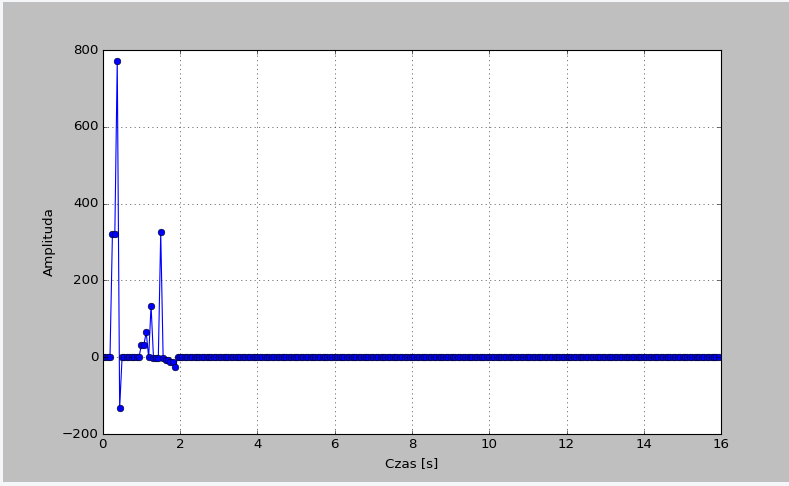
\includegraphics[width=1\textwidth]{img/walshs1.png}
                    \caption{Wykresy dla sygnału S1}
                \end{figure}
                \FloatBarrier

                Czas wykonania obliczeń (s): 0.029 
            
            \subsubsection{Szybka transformacja Walsha-Hadamarda}

            
                \begin{figure}[h!]
                    \centering
                    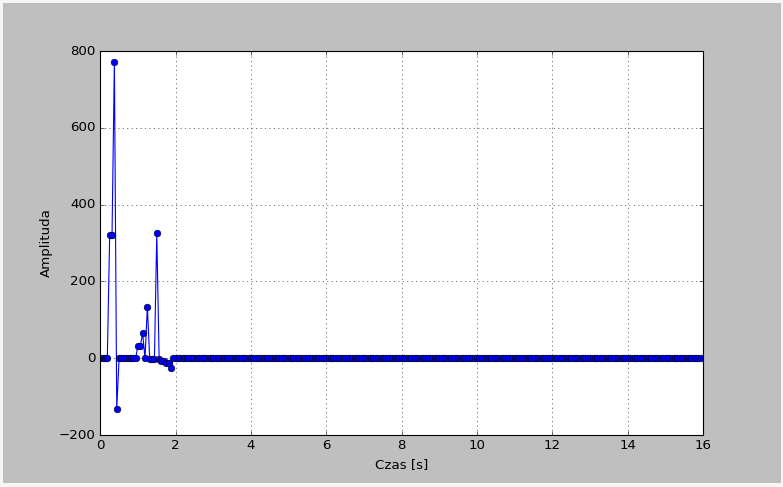
\includegraphics[width=1\textwidth]{img/fwalshs1.png}
                    \caption{Wykresy dla sygnału S1}
                \end{figure}
                \FloatBarrier

                Czas wykonania obliczeń (s): 0.001  

    
    \subsection{Sygnał S2} 

        \begin{table}[h!]
            \centering
            \begin{tabular}{|l|l|l|}
                \hline
                Czas początkowy & \shortstack{Czas trwania \\ sygnału} & \shortstack{Częstotliwość\\ próbkowania}   \\ \hline
                0 & 16s & 16Hz         \\ \hline
            \end{tabular}
            \caption{Parametry wejściowe dla sygnału S2}
        \end{table}

        \begin{figure}[h!]
            \centering
            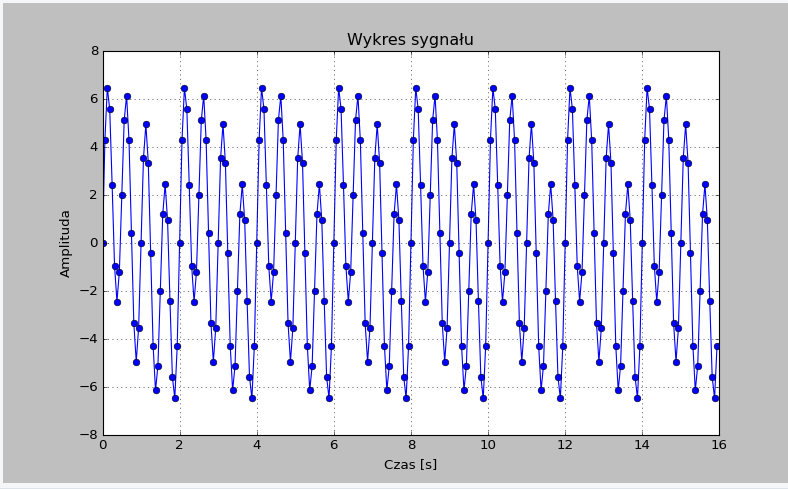
\includegraphics[width=\textwidth]{img/S2.png}
            \caption{Wykres sygnału S2}
        \end{figure}
        \FloatBarrier

        \subsubsection{Dyskretna tranformacja Fouriera z definicji}

                \FloatBarrier
                \begin{figure}[h!]
                    \centering
                    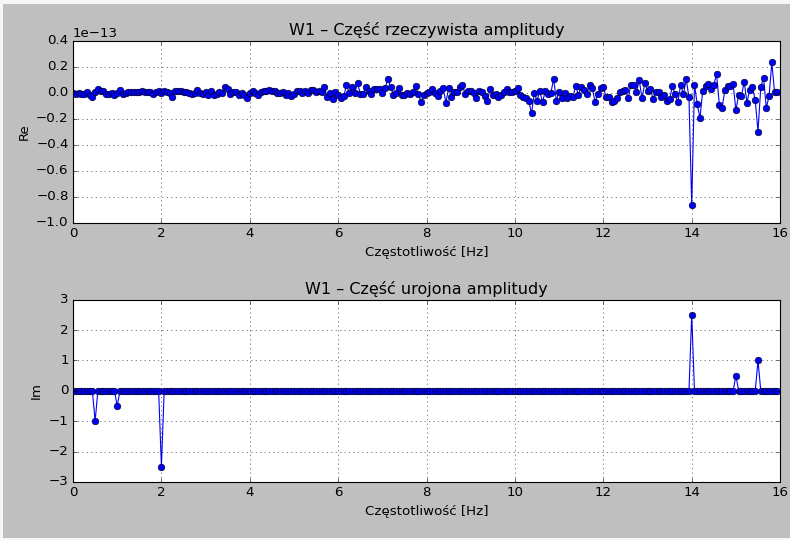
\includegraphics[width=1\textwidth]{img/w1s2.png}
                    \caption{Wykresy W1 dla sygnału S2}
                \end{figure}

                \begin{figure}[h!]
                    \centering
                    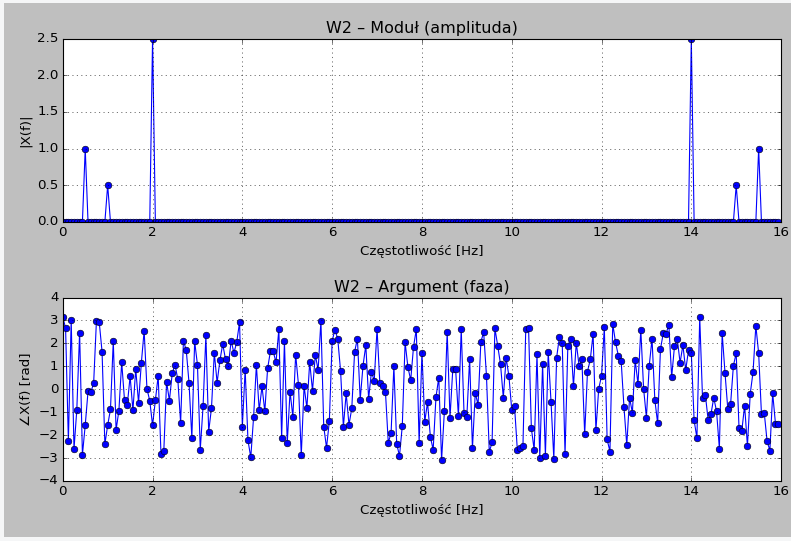
\includegraphics[width=1\textwidth]{img/w2s2.png}
                    \caption{Wykresy W2 dla sygnału S2}
                \end{figure}
                \FloatBarrier

                Czas wykonania obliczeń (s): 0.021

        \subsubsection{Szybka tranformacja Fouriera}

                \FloatBarrier
                \begin{figure}[h!]
                    \centering
                    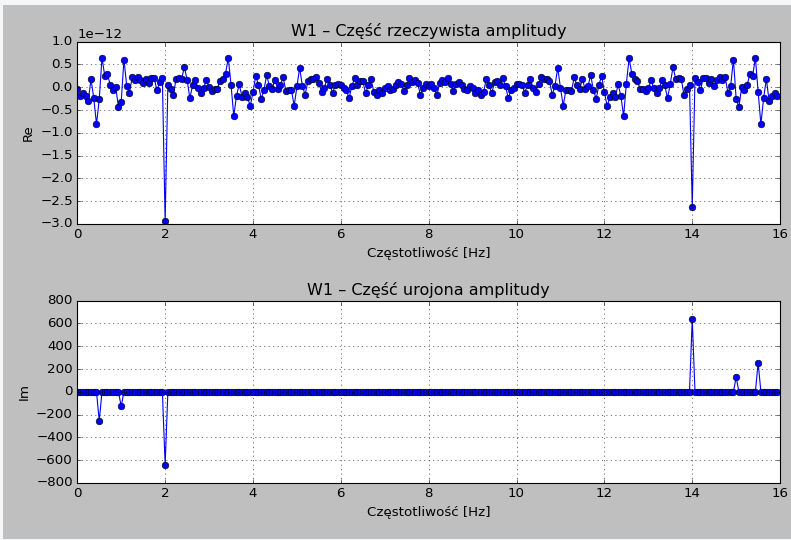
\includegraphics[width=1\textwidth]{img/w1s2_2.png}
                    \caption{Wykresy W1 dla sygnału S2}
                \end{figure}

                \begin{figure}[h!]
                    \centering
                    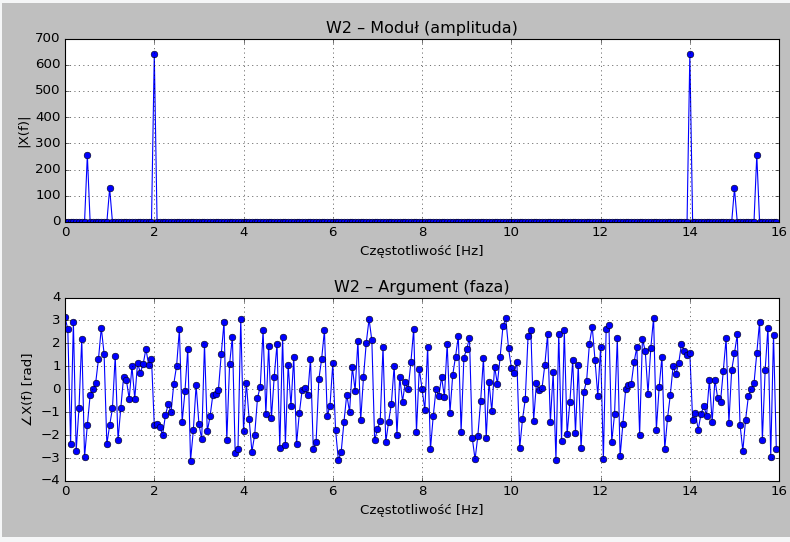
\includegraphics[width=1\textwidth]{img/w2s2_2.png}
                    \caption{Wykresy W2 dla sygnału S2}
                \end{figure}
                \FloatBarrier

                Czas wykonania obliczeń (s): 0.002

            \subsubsection{Transformacja kosinusowa z definicji}

            
                \begin{figure}[h!]
                    \centering
                    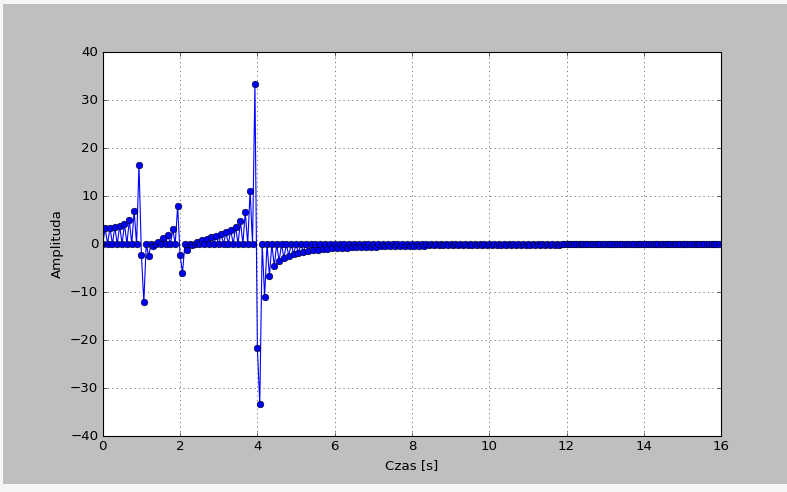
\includegraphics[width=1\textwidth]{img/dcts2.png}
                    \caption{Wykresy dla sygnału S2}
                \end{figure}
                \FloatBarrier

                Czas wykonania obliczeń (s): 0.026
            
            \subsubsection{Transformacja Walsha-Hadamarda z definicji}

            
                \begin{figure}[h!]
                    \centering
                    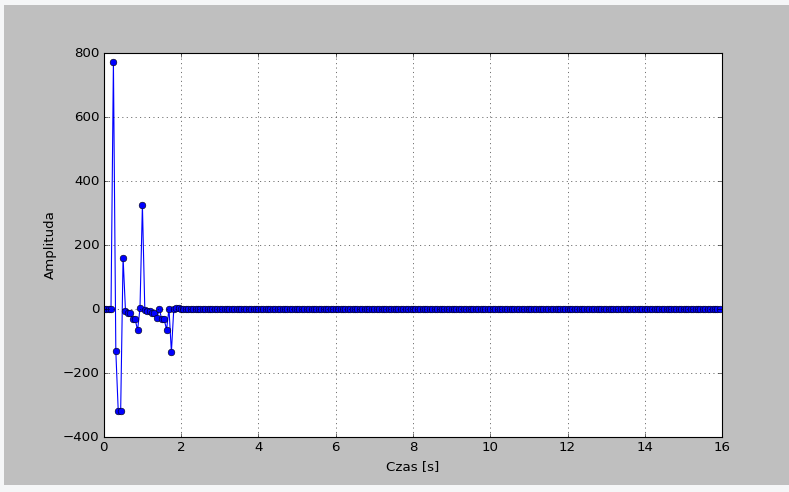
\includegraphics[width=1\textwidth]{img/walshs2.png}
                    \caption{Wykresy dla sygnału S2}
                \end{figure}
                \FloatBarrier

                Czas wykonania obliczeń (s): 0.025 
            
            \subsubsection{Szybka transformacja Walsha-Hadamarda}

            
                \begin{figure}[h!]
                    \centering
                    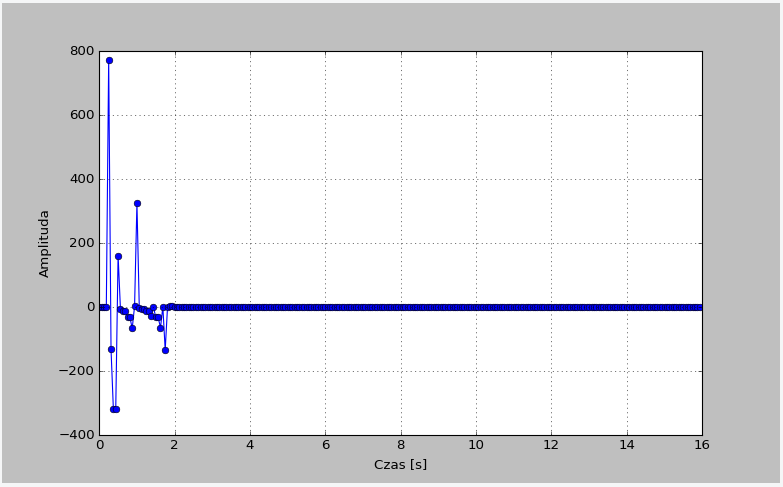
\includegraphics[width=1\textwidth]{img/fwalshs2.png}
                    \caption{Wykresy dla sygnału S2}
                \end{figure}
                \FloatBarrier

                Czas wykonania obliczeń (s): 0.002 

    \subsection{Sygnał S3} 

        \begin{table}[h!]
            \centering
            \begin{tabular}{|l|l|l|}
                \hline
                Czas początkowy & \shortstack{Czas trwania \\ sygnału} & \shortstack{Częstotliwość\\ próbkowania}   \\ \hline
                0 & 16s & 16Hz         \\ \hline
            \end{tabular}
            \caption{Parametry wejściowe dla sygnału S3}
        \end{table}

        \begin{figure}[h!]
            \centering
            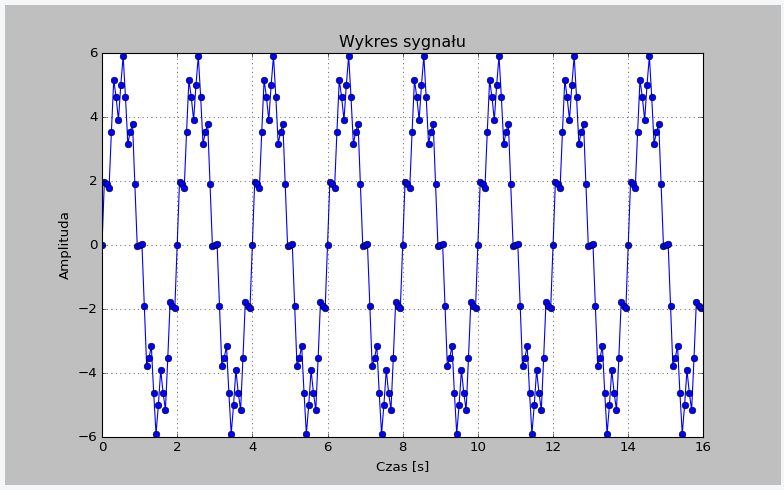
\includegraphics[width=\textwidth]{img/S3.png}
            \caption{Wykres sygnału S3}
        \end{figure}
        \FloatBarrier

        \subsubsection{Dyskretna tranformacja Fouriera z definicji}

                \FloatBarrier
                \begin{figure}[h!]
                    \centering
                    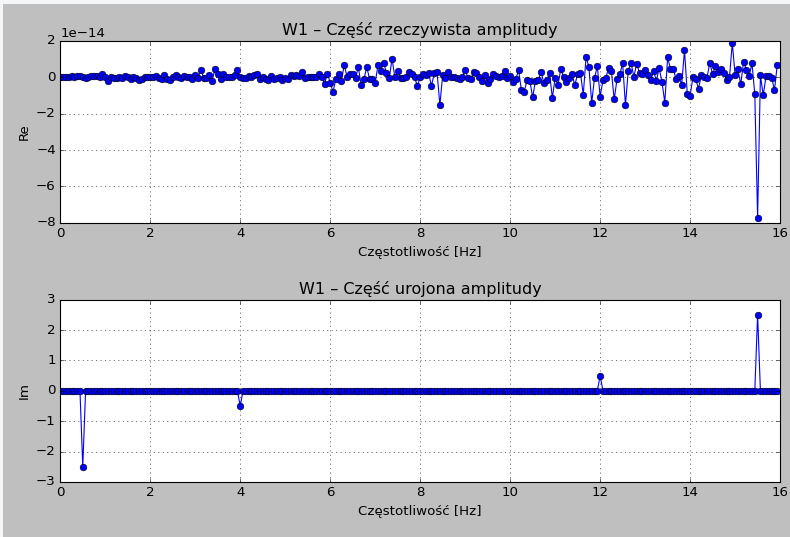
\includegraphics[width=1\textwidth]{img/w1s3.png}
                    \caption{Wykresy W1 dla sygnału S3}
                \end{figure}

                \begin{figure}[h!]
                    \centering
                    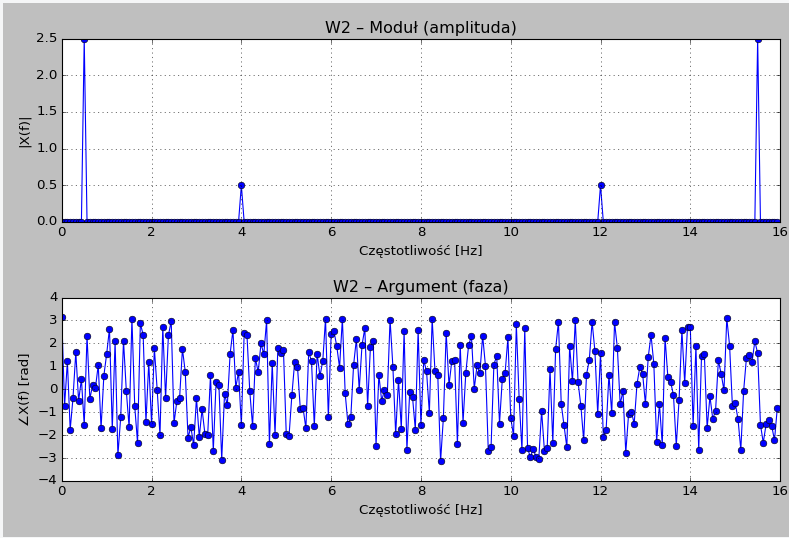
\includegraphics[width=1\textwidth]{img/w2s3.png}
                    \caption{Wykresy W2 dla sygnału S3}
                \end{figure}
                \FloatBarrier

                Czas wykonania obliczeń (s): 0.015

        \subsubsection{Szybka tranformacja Fouriera}

                \FloatBarrier
                \begin{figure}[h!]
                    \centering
                    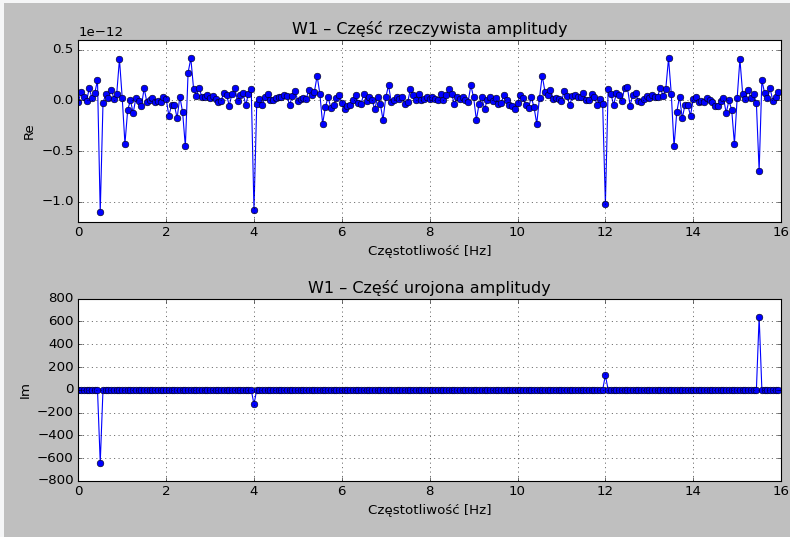
\includegraphics[width=1\textwidth]{img/w1s3_2.png}
                    \caption{Wykresy W1 dla sygnału S3}
                \end{figure}

                \begin{figure}[h!]
                    \centering
                    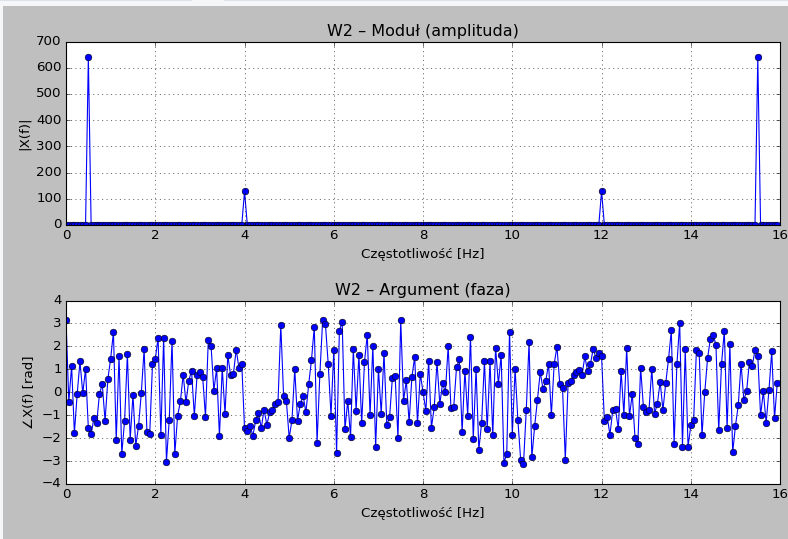
\includegraphics[width=1\textwidth]{img/w2s3_2.png}
                    \caption{Wykresy W2 dla sygnału S3}
                \end{figure}
                \FloatBarrier

                Czas wykonania obliczeń (s): 0.001

            \subsubsection{Transformacja kosinusowa z definicji}

            
                \begin{figure}[h!]
                    \centering
                    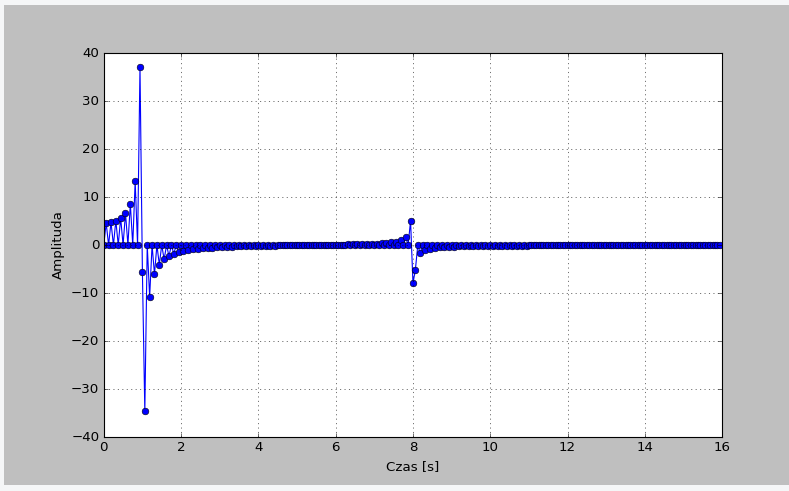
\includegraphics[width=1\textwidth]{img/dcts3.png}
                    \caption{Wykresy dla sygnału S3}
                \end{figure}
                \FloatBarrier

                Czas wykonania obliczeń (s): 0.024
            
            \subsubsection{Transformacja Walsha-Hadamarda z definicji}

            
                \begin{figure}[h!]
                    \centering
                    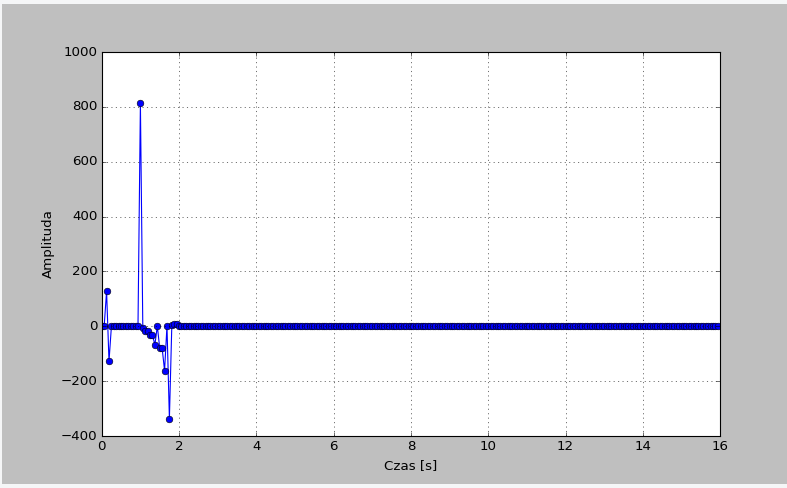
\includegraphics[width=1\textwidth]{img/walshs3.png}
                    \caption{Wykresy dla sygnału S3}
                \end{figure}
                \FloatBarrier

                Czas wykonania obliczeń (s): 0.026 
            
            \subsubsection{Szybka transformacja Walsha-Hadamarda}

            
                \begin{figure}[h!]
                    \centering
                    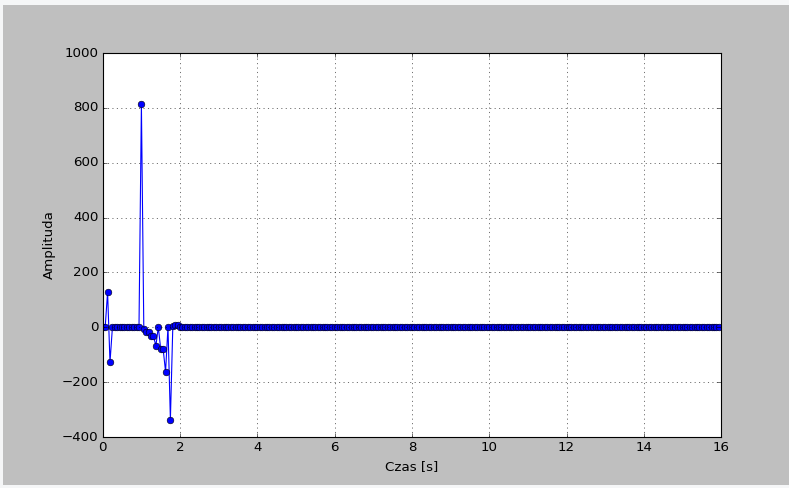
\includegraphics[width=1\textwidth]{img/fwalshs3.png}
                    \caption{Wykresy dla sygnału S3}
                \end{figure}
                \FloatBarrier

                Czas wykonania obliczeń (s): 0.001 
    \subsection{Tabela czasu wykonywania obliczeń}
        \begin{table}[h!]
            \begin{tabular}{|l|l|l|l|}
                \hline
                                                                            & S1        & S2     & S3        \\ \hline
                Dyskretna tranformacja Fouriera z definicji                 & 0.020     & 0.021  & 0.015     \\ \hline
                Szybka tranformacja Fouriera                                & 0.002     & 0.002  & 0.001     \\ \hline
                Transformacja kosinusowa z definicji                        & 0.045     & 0.026  & 0.024     \\ \hline
                Transformacja Walsha-Hadamarda z definicji                  & 0.029     & 0.025  & 0.026     \\ \hline
                Szybka transformacja Walsha-Hadamarda                       & 0.001     & 0.002  & 0.001     \\ \hline
            \end{tabular}
        \end{table}
    }
\section{Dyskusja i wnioski}
        Eksperymenty zostały podzielone na trzy grupy, każda grupa
        przedstawia wyniki transformacji jedego z sygnałów S1, S2 i
        S3. Większa liczba eksperymentów pozwala lepiej potwierdzić
        wysnuwane wnioski, które są w tym przypadku takie same, dla
        każdej serii doświadczeń.

        Jeżeli chodzi o wyniki transformacji, to wydają się one
        być poprawne dla wszystkich przeprowadzonych eksperymentów, w
        wynikach transformacji Fouriera, kosinusowej i
        Walsha-Hadamarda, zawsze można odnaleźć tyle składowych, ile
        rzeczywiście tworzyło transformowaną funkcję. I tak kolejno
        dla serii eksperymentów znaleziono 2, 3 i znowu 2 składowe.
        Warto jeszcze wspomnieć, że wyniki transformacji Fouriera,
        która była przeprowadzana różnymi metodami, również różnią się
        od siebie. Widać, że dla każdej z dwóch metod część
        rzeczywista wyniku wygląda innaczej. Natomiast moduł zawsze
        wygląda tak samo i jako, że jest przeniesiony w dziedzinę
        częstotliwości a oś X odpowiednie przeskalowana, pozwala
        bezpośrednio odczytać, jakie częstotliwości składowe tworzyły
        transformowany sygnał. Oczywiście należy pamiętać, że druga
        połowa (w osi X) wykresu jest zawsze symetryczna do pierwszej
        i nie niesie dodatkowej informacji.

        Ostatnim rozważanym aspektem jest czas obliczeń. Pierwszym
        oczywistym wnioskiem potwierdzonym przez prawie wszystkie
        doświadczenia jest to, że algorytmy
        szybkie działają znacznie szybciej, niż algorytmy zbudowane na
        podstawie definicji. Widać to wyraźnie na przykładach
        transformacji Walsha-Hadamarda oraz kosinusowej. 
        FFT okazała się za każdym razem około
        dziesięciokrotnie szybsza niż transformacja z definicji. 
        W przypadku transformacji Walsha-Hadamarda ponad
        trzydzieści razy. Warto zwrócić tutaj uwagę, że w ogóle
        transformacja Walsha-Hadamarda okazała się najszybsza, druga w
        kolejności jest transformacjakosinusowa, najwolniejsza natomiast jest
        transformacja Fouriera. Należy wziąc pod uwagę, że
        zależności pomiędzy czasem trwania różnych algorytmów zmienią
        się dla większej bądź mniejszej liczby próbek. Zysk czasowy,
        który otrzymujemy dla algorytmów szybkich, zawsze jest coraz
        bardzie zauważalny przy obliczeniach, na większej ilości
        danych. Ponadto trzeba wspomnieć, że czas obliczeń może
        zmieniać się w zależności od chwilowego obciążenia procesora
        komputera i konkretnych szczegółów implementacyjnych, które
        nie są charakterystyczne dla algorytmu ale dla danej jego
        implementacji.
    
    

%%%%%%%%%%%%%%%%%%%%%%%%%%%%%%%%%%%%%%%%%%%%%%%%%%%%%%%%%%%%%%%%%%%%%%%%%%%%%%%%%%%%%%%%%%%%%%%%%%%%%%%%%%%%%%%%%
% BIBLIOGRAFIA
%%%%%%%%%%%%%%%%%%%%%%%%%%%%%%%%%%%%%%%%%%%%%%%%%%%%%%%%%%%%%%%%%%%%%%%%%%%%%%%%%%%%%%%%%%%%%%%%%%%%%%%%%%%%%%%%%

\begin{thebibliography}{9}

    \bibitem{instrukcja}
    Politechnika Łódzka, 
    \emph{Instrukcja do zadania 4}, 
    Dostęp online: \url{https://ftims.edu.p.lodz.pl/mod/url/view.php?id=6495}, 
    [dostęp: 10 maja 2025].


    \bibitem{python-doc}
    Python Software Foundation, 
    \emph{Python Documentation}, 
    Dostęp online: \url{https://docs.python.org/3/}, 
    [dostęp: 10 maja 2025].

    \bibitem{tkinter-doc}
    Python Software Foundation, 
    \emph{Tkinter Documentation}, 
    Dostęp online: \url{https://docs.python.org/3/library/tkinter.html}, 
    [dostęp: 10 maja 2025].

\end{thebibliography}

\end{document}
